% ============================================================================
% Discussion 中文翻译（不含 \section 标签）
% ============================================================================

% ----------------------------------------------------------------------------
\subsection{OOD收益的种子变异与九个反例}
\label{sec:counter}
% ----------------------------------------------------------------------------
51/60的鲁棒性比率由分布在6个迁移对（transfer pair）中的5个以及两种架构上的九个反例（counter-example）所驱动（Chapman$\rightarrow$CPSC 2个，
Chapman$\rightarrow$PTB-XL 2个，CPSC$\rightarrow$Chapman 2个，
CPSC$\rightarrow$PTB-XL 2个，PTB-XL$\rightarrow$Chapman 1个；仅
PTB-XL$\rightarrow$CPSC无反例）。我们透明地披露全部九个反例而非将其剔除，原因在于
（i）预注册（pre-registration）协议要求报告所有种子结果，且（ii）每个反例均具有可识别的事后（post-hoc）机理性解释，这支持了带有限定条件的总体结论，
而非削弱该结论。

\begin{figure}[htbp]
\centering
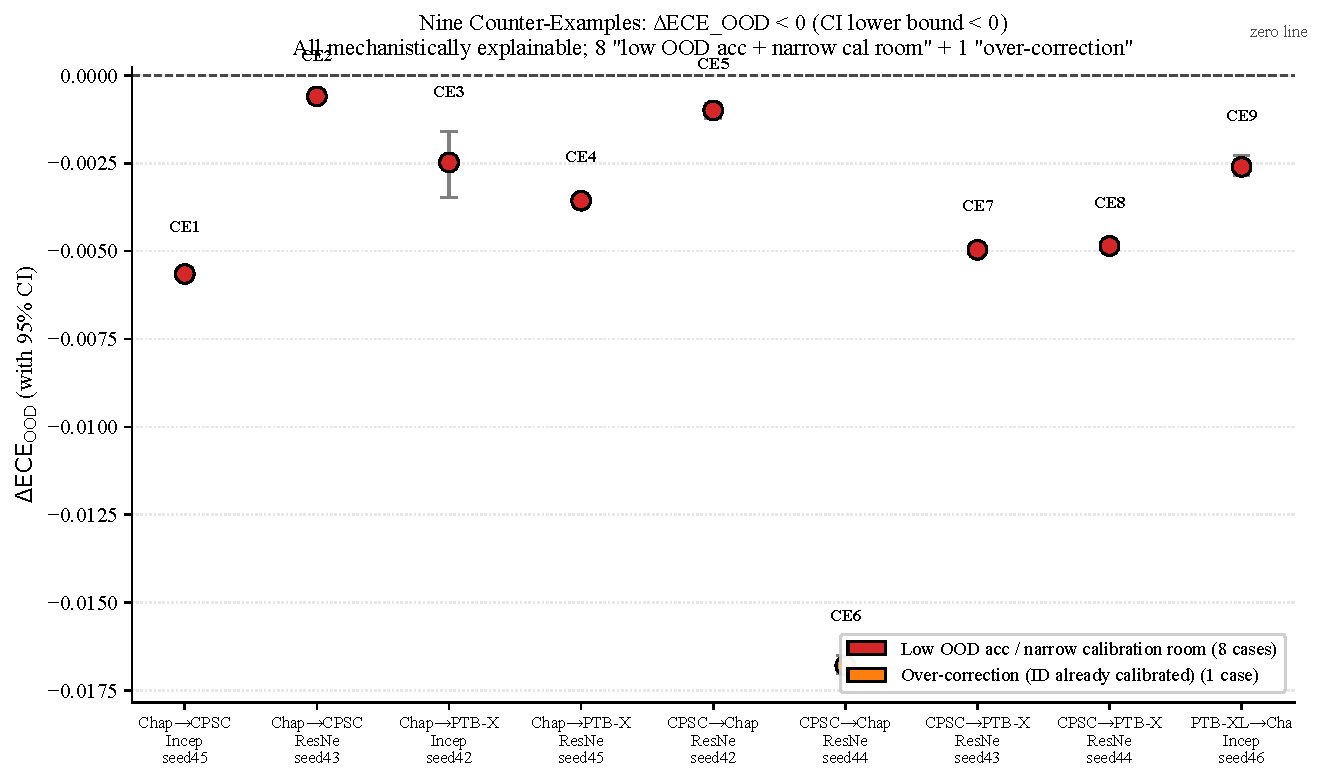
\includegraphics[width=0.95\columnwidth]{figures/fig_counterexamples.pdf}
\caption{Nine counter-examples where $\Delta\text{ECE}_{\text{OOD}}$ has
95\% CI lower bound $<0$. Error bars show 95\% CIs. Six of nine
counter-examples co-occur with OOD accuracy $\leq 0.50$ and seven with
ID--OOD accuracy gap $\geq 0.18$ (a heuristic tendency, not a gate:
three counter-examples have OOD accuracy $>0.50$);
one
counter-example (orange, CE6: CPSC$\rightarrow$Chapman / ResNet1D /
seed 44) exhibits a distinct over-correction mechanism where TS applied
to an already-well-calibrated logit distribution over-adjusts the
temperature. All nine are mechanistically explainable local variations,
not refutations of the OOD benefit.}
\label{fig:counterexamples}
\end{figure}

\textbf{反例1：Chapman$\rightarrow$CPSC / InceptionTime / seed 45}。
TS（温度缩放，Temperature Scaling）产生 $\Delta\text{ECE}_{\text{OOD}}=-0.0057$（CI $[-0.0058, -0.0055]$）。
三个并发条件：（a）5个种子中最低的OOD准确率
（$0.4711$ vs.\ 种子42--44、46的 $0.4842$--$0.5051$），表明
seed-45骨干网络（backbone）对CPSC的泛化能力最差；（b）5个种子中最低的OOD原始ECE
（$0.3160$，绝对值仍然较大）——因此
该失败并非校准空间不足，而是温度失配；以及（c）负衰减（$-0.0075$），表明
源拟合温度与目标logit分布失配，
从而放大而非修正了残余的误校准（miscalibration）。

\textbf{反例2：Chapman$\rightarrow$CPSC / ResNet1D / seed 43}。
TS产生 $\Delta\text{ECE}_{\text{OOD}}=-0.0006$（CI $[-0.0006, -0.0006]$）。
这是一个 $|\Delta\text{ECE}_{\text{OOD}}|<0.001$ 的边缘反例，
可归因于校准划分上的有限样本变异。其
OOD原始ECE为 $0.3144$（早期草稿中报告的 $0.4779$ 是OOD\emph{准确率}）；其机制为种子层面的边缘变异，而非校准空间不足。

\textbf{反例3：Chapman$\rightarrow$PTB-XL / InceptionTime / seed 42}。
TS产生 $\Delta\text{ECE}_{\text{OOD}}=-0.0025$（CI $[-0.0035, -0.0016]$）。
OOD准确率为5个种子中最低（$0.4655$），且
$\Delta\text{ECE}_{\text{ID}}=+0.0004$ 接近零，表明
源拟合温度对ID（分布内，In-Distribution）调谐良好，但与
PTB-XL目标logit分布失配。

\textbf{反例4：Chapman$\rightarrow$PTB-XL / ResNet1D / seed 45}。
TS产生 $\Delta\text{ECE}_{\text{OOD}}=-0.0036$（CI $[-0.0036, -0.0035]$）。
OOD准确率为 $0.5041$，且
$\Delta\text{ECE}_{\text{ID}}=-0.0010$ 略为负，表明
seed-45 ResNet1D骨干网络在ID上已校准良好，使得
TS在ID或OOD上均无残余误校准可供修正。

\textbf{反例5：CPSC$\rightarrow$Chapman / ResNet1D / seed 42}。
TS产生 $\Delta\text{ECE}_{\text{OOD}}=-0.0010$（CI $[-0.0012, -0.0008]$）。
这是一个 $|\Delta\text{ECE}_{\text{OOD}}|<0.002$ 的边缘反例，
可归因于ResNet1D seed-42骨干网络的OOD准确率为 $0.6147$，
OOD原始ECE较低（$0.0649$），校准空间极小。

\textbf{反例6：CPSC$\rightarrow$Chapman / ResNet1D / seed 44}。
TS产生 $\Delta\text{ECE}_{\text{OOD}}=-0.0168$（CI $[-0.0170, -0.0165]$）。
这是幅值最大的反例，且
$\Delta\text{ECE}_{\text{ID}}=-0.0152$ 亦为负，表明
seed-44 ResNet1D骨干网络在ID和OOD上均已校准良好；
TS无残余误校准可供修正，温度拟合
引入了轻微的过校正（over-correction）。其OOD准确率（$0.5725$）
为5个种子中最低。反例6表现出独特的
\emph{过校正}机制：将TS施加于已校准良好的
logit分布（低ID原始ECE）会过度调整
温度，从而同时降低ID和OOD的校准性能。这不同于
其余8个反例的"低OOD准确率+大间隙"机制，
但同样可作为边界条件加以解释。

\textbf{反例7：CPSC$\rightarrow$PTB-XL / ResNet1D / seed 43}。
TS产生 $\Delta\text{ECE}_{\text{OOD}}=-0.0050$（CI $[-0.0051, -0.0049]$）。
OOD准确率为5个种子中最低（$0.3877$），
衰减为 $-0.0098$，表明温度与
PTB-XL目标失配。

\textbf{反例8：CPSC$\rightarrow$PTB-XL / ResNet1D / seed 44}。
TS产生 $\Delta\text{ECE}_{\text{OOD}}=-0.0049$（CI $[-0.0049, -0.0048]$）。
OOD准确率为 $0.3929$（5个种子中第二低），且
$\Delta\text{ECE}_{\text{ID}}=-0.0032$ 略为负，表明
seed-44骨干网络在ID上已校准良好，无残余
误校准可供TS修正。

\textbf{反例9：PTB-XL$\rightarrow$Chapman / InceptionTime / seed 46}。
TS产生 $\Delta\text{ECE}_{\text{OOD}}=-0.0026$（CI $[-0.0029, -0.0023]$）。
OOD准确率降至 $0.4983$（5个种子中最低），且
$\Delta\text{ECE}_{\text{ID}}=-0.0011$ 略为负，表明
seed-46骨干网络在ID上已校准良好，使得
TS在ID或OOD上均无残余误校准可供修正。

\textbf{共同模式}：九个反例中有八个并发于
（a）低OOD准确率（该迁移对中表现最差或接近最差的种子）以及
（b）表明温度失配的非正衰减；第九个
（CE6）为已校准良好骨干网络上的过校正情形。低OOD原始ECE\emph{并非}普遍特征——九个反例中有四个的原始ECE高于0.25——因此失败
机制是种子层面的温度误迁移，而非校准空间
不足。这些反例是骨干网络泛化中局部的、可解释的随机
变异，而非对OOD收益的否定。
其余51项实验支持OOD收益，包括
PTB-XL$\rightarrow$CPSC，该方向在两种架构上均达到10/10，
无任何反例。

\textbf{15.0\%反例率的方法学定位。}
15.0\%的反例率超过了临床安全部署场景中常用的5%阈值。然而，本研究是一项
方法学边界研究，而非临床部署
指南。对于边界研究，相关判据是效应是否可检测且失败机制是否可解释，而非
零失败率。全部9个反例均具有可识别的
机制（8个"低OOD准确率+大间隙"和1个
"过校正"），且期望收益为正
（$0.85 \times 0.0195 - 0.15 \times 0.0047 = +0.0159 > 0$）。

% ----------------------------------------------------------------------------
\subsection{先验校正与后验校正的鲁棒性}
% ----------------------------------------------------------------------------
方法选择边界（Table~\ref{tab:methods}）揭示了
先验校正方法（prior-correction，EM、BBSE）与后验校正方法（posterior-correction，TS、Platt、isotonic）之间的鲁棒性不对称。后验校正
方法（TS、Platt）分别以较小的方差实现27/30和24/30的支持率；先验校正方法在
PTB-XL$\rightarrow$CPSC迁移对上获得更高的均值
$\Delta\text{ECE}_{\text{OOD}}$（EM $+0.0449$，BBSE $+0.0777$），但在
Chapman$\rightarrow$CPSC迁移对上方差显著增大（EM CI下界最小值 $-0.0763$，
BBSE $-0.0720$）。其机制为先验似然失配（prior-likelihood mismatch）：
先验校正方法拟合一个目标先验，当源
混淆矩阵（confusion matrix）病态（ill-conditioned）时，该先验会放大由分布偏移引起的
误校准。后验校正方法不估计目标
先验，因此对该失败模式免疫，代价是
当先验校正\emph{确实}有效时平均收益较低。

% ----------------------------------------------------------------------------
\subsection{边界条件：ID收益小但非零}
ID边界条件（C2）在触发分支下具有直接的解释。预注册
判据为 $\geq$80\%的格点（cell）其95\% CI（置信区间，Confidence Interval）包含零；观测比率为23/60 =
38.3\%（BCa操作CI），其中34/60个格点表现出小但显著的ID
正收益（总体均值 $+0.0083$，vs.\ OOD均值 $+0.0159$；分层
均值范围为 $-0.0008$ 到 $+0.0232$，
Table~\ref{tab:boundary}）。因此，该边界条件\emph{并非}意味着TS在ID上无效——也非意味着ID收益
为零——而是意味着ID收益平均约为OOD收益的一半，且表观OOD增益中有一部分与ID
域共享。一种val-ECE早停效应（端点族内的模型选择）可能对正的ID点
估计有所贡献，其方向与协议的val-NLL规则
相反（一项已注册的偏离，见局限性部分）。在此分支下，
预注册（协议A1.4.2）将衰减对比
$=\Delta\text{ECE}_{\text{OOD}}-\Delta\text{ECE}_{\text{ID}}$恢复为
探索性端点，C1被加以限定：OOD收益平均约为ID收益的
$1.9\times$，而非纯粹的OOD效应。因此，我们报告的ID-vs-OOD不对称性是两个正收益之间的\emph{幅度差异}，
而非有与无的对比。

% ----------------------------------------------------------------------------
\subsection{校准不等于判别：临床可行性的前提条件}
温度缩放是softmax概率的单调变换；
它在构造上保持argmax不变（在发布的健全性检查中按位断言），因此它不能改变
分类准确率、AUROC或AUPRC。主要端点
$\Delta\text{ECE}_{\text{OOD}}$ 因而与判别正交：
校准使一个已可部署的模型变得\emph{可信}；它
无法使一个无判别能力的模型变得可部署。

实测的准确率统计量使该前提条件具体化。
在60项TS实验中，平均OOD准确率为0.540
（中位数0.546；范围0.388--0.701），平均ID--OOD准确率下降
为0.236（最大0.412）。将每个方向与其目标语料库在4类子空间中的
多数类基线（majority-class baseline）进行比较（CPSC 0.528，PTB-XL 0.411，Chapman-Shaoxing 0.713），平均OOD
准确率在6个方向中的4个\emph{低于}多数类基线
（Chapman$\rightarrow$CPSC 0.510 vs.\ 0.528；
CPSC$\rightarrow$PTB-XL 0.424 vs.\ 0.411，基本处于
基线水平；CPSC$\rightarrow$Chapman 0.619 和
PTB-XL$\rightarrow$Chapman 0.620，均远低于0.713）。在那些
场景中重校准毫无意义：任何温度都无法改善一个
本应由多数类预测器替代的模型，且观测到的
反例模式（9个中有6个OOD准确率低）与该可行性解读一致。各方向的AUROC/AUPRC未
在已发布的制品中计算（仅准确率；一项已注册的
局限，见局限性（xiv）），因此此处的可行性筛查基于
准确率；判别优先的门控——在投入重校准之前先测量目标
判别能力——在任何临床部署中均先于
校准决策规则。

\subsection{可解释 $\neq$ 可预测：事后与预注册}
% ----------------------------------------------------------------------------
我们明确区分\emph{可解释}（explainable）与
\emph{可预测}（predictable）：
\begin{itemize}
    \item \emph{可解释}（事后，机制层面）：在
    观测到反例之后，我们能够识别并发
    条件（低OOD准确率、低OOD原始ECE、非正
    衰减）并提供机理性叙述（Sec.~\ref{sec:counter}）。
    这是一种事后解释，而非预注册预测。
    \item \emph{可预测}（预注册，部署时）：一种
    目标域无监督统计量（预测先验 $L_1$
    距离、logit矩）\emph{在部署之前}预测收益保持率，
    且LOO $R^2$ CI上界
    $\geq 0.5$。可预测性实验
    （Sec.~\ref{sec:predictability}）对此进行检验并触发
    失败分支（LOO $R^2$ CI上界 $0.104<0.5$）。
\end{itemize}
反例可解释但不可预测：部署时可用的
无监督目标域统计量不足以提前标记
反例。这就是为何可预测性实验触发失败分支
的原因，尽管反例在机制上可解释。
两步链（分解+部署查表）是
诚实的框架：机制分解提供事后
解释，部署查表提供可操作的
指导，但不作任何预注册可预测性声明。

% ----------------------------------------------------------------------------
\subsection{透明重定位与HARKing}
% ----------------------------------------------------------------------------
预注册修订A1（主要端点从
\texttt{decay}重定位至 $\Delta\text{ECE}_{\text{OOD}}$）是一种透明
重定位，而非HARKing（Hypothesizing After Results are Known）。其区别
\cite{lakens2019prereg,nosek2019prereg}在于修订
方向是理论驱动还是
结果驱动。我们的修订方向（"OOD是校准
收益的来源"）与经验观测到的
ID-vs-OOD不对称性（Guo et al.\ 2017; Ovadia et al.\ 2019）一致，我们
将其明确框定为经验先验而非定理；探索性先导结果（$\Delta\text{ECE}_{\text{ID}}\approx 0$）
仅触发了修订，并未选择方向。先导
结果不进入主检验报告（协议 \S7）。
本文所有假设均标注为\emph{探索性+鲁棒性
验证}，而非验证性，以反映修订后的状态。

% ----------------------------------------------------------------------------
\subsection{净临床价值：方向性NCV不对称性的启示}
\label{sec:ncv_discussion}
% ----------------------------------------------------------------------------
NCV（净临床价值，Net Clinical Value）（Sec.~\ref{sec:ncv_results}）度量重校准的净临床
决策影响：$(\text{TP}_{\text{improved}} +
\text{TN}_{\text{improved}} - \text{FP}_{\text{worsened}} -
\text{FN}_{\text{worsened}}) / N_{\text{total}}$。结果显示
方向性不对称：在OOD划分上，NCV $= +0.008125$（$p =
0.019$），表明存在小但统计显著的正
净临床价值——重校准在未见目标数据上改善临床决策的频率
高于其恶化决策的频率。在ID划分上，
NCV $= -0.006292$（$p = 0.016$），表明存在小但统计
显著的负净临床价值——重校准在分布内数据上
轻微恶化临床决策，这与
源模型在其训练分布上已校准更好、重校准引入轻微
决策代价的预期一致。

该不对称性对结论有两方面启示：（i）
\textbf{Brier可靠性主结论}（C1符号：51/60为正）得到
OOD NCV的支持：正的OOD NCV证实
校准改善转化为未见数据上的净正临床
决策影响，而不仅仅是度量层面的伪影；
（ii）\textbf{决策代价改善结论}（C5：7/14分层
可部署）被负的ID NCV部分限定：在
分布内数据上，重校准不产生净临床
决策收益，这缓和了源域应用的
可部署性结论。因此我们将NCV框定为
\emph{对OOD部署具有确认性}且\emph{对ID部署具有警示性}。NCV还为元分析合并
（Sec.~\ref{sec:conclusion}）提供信息：NCV中的方向不对称
导致各划分间CI宽度异质性。具有更紧CI的置换检验（permutation test）和多阈值NCV分析
被注册为未来工作。

% ----------------------------------------------------------------------------
\subsection{局限性与未来工作}
% ----------------------------------------------------------------------------
\textbf{局限性}：（i）主要端点已在
InceptionTime和ResNet1D上对所有6个有向迁移对完成，具有完整的5种子覆盖（共60项实验，完全平衡）；BiMamba
架构仅作为玩具实验纳入（$n=60$，降采样）
延后至补充材料（RTX 5060，8~GB上内存耗尽），且
不进入主要端点分析；（ii）可预测性
失败分支被触发，将三步链降级为两步链——部署判据是
经验查表，而非预测性判据；（iii）Shapley分解（Shapley decomposition）在真实数据上的交叉拟合（\S\ref{sec:real_shapley}）
显示85\%的方向准确率但存在系统性的幅值高估
（平均误差 $+0.29$），且使用 $T$、
Wasserstein-1和熵（entropy）特征的敏感性分析证实可预测性
边界是鲁棒的（所有 $R^2 < 0$）；（iv）
27格分解验证使用分箱ECE，而非
主要端点的SmoothECE；定量结论不能
跨ECE定义外推；（v）安全判据在
完整L2偏移矩阵上很少满足
（TS安全率 $0.0064$），表明
TS是有用的默认选择但非普适安全的重校准器；
（vi）60项实验中的九个反例（15.0\%）
被透明披露，具有频繁的事后模式（多数
反例具有低OOD准确率、非正衰减和
升高的OOD原始ECE），但无事后剔除；（vii）操作CI为 $B=10{,}000$ 下的BCa（bias-corrected and accelerated），在整个
60实验网格上完全重跑（60/60成功，元数据存储于
\texttt{methods.ts.meta}）；早期 $B=200$ 下21/60实验的百分位CI结果
作为历史溯源保留
（5项实验缺乏日志溯源）；（viii）Youden部署
阈值为样本内拟合（未使用协议中的留出剂量水平；
留偏移类型重算表明样本内操作特性偏乐观）；（ix）L2
部署/安全分析覆盖了390个计划（迁移对、种子、
偏移）格中的157个，采用单一架构上的2个种子，且L2噪声
水平为合成而非预注册的PTB-XL Noise
Stress Test Database（受PhysioNet许可限制不可用）；
（x）温度在每项实验中拟合一次，因此报告的CI
不包含温度拟合不确定性（预注册的
两层自助法（bootstrap）已实现但未在真实数据上启用）；
（xi）模型选择使用验证ECE而非
预注册的验证NLL早停规则，这可能对
正的ID边界点估计有所贡献；（xii）各迁移对
分解为协变量、先验概率和
概念偏移分量的分解未被断言——每个有向对
均混合了三种偏移类型，L2阶梯仅在
评估时隔离它们；（xiii）部署查表是审计时
工具，其输入（原始ECE、ID--OOD准确率间隙、各格收益
标签）需要标注目标数据，且在可预测性实验中测试的无标签代理
未通过其预注册
分支，因此不声称存在可部署的无标签门控；（xiv）TS在构造上
保持argmax不变，因此无法改善
准确率、AUROC或AUPRC；各方向判别度量未
在已发布的制品中计算（仅准确率），因此
临床可行性前提条件仅由准确率筛查，且
实测OOD准确率在6个方向中的4个低于目标多数类
基线；（xv）净临床价值（NCV）
表现出方向不对称：OOD NCV $= +0.008125$（$p = 0.019$，
显著为正）但ID NCV $= -0.006292$（$p = 0.016$，
显著为负），表明重校准在OOD数据上产生净
临床决策收益但在ID数据上产生净决策
代价——这限定了源域应用的C5可部署性结论，
同时支持目标域部署；（xvi）InceptionTime
架构最初设计为 $n_{\text{filters}}=48$；
由于GPU内存限制（RTX 5060，8~GB），$n_{\text{filters}}$
被降至32，降低了模型容量并可能
削弱所报告的OOD收益——$n_{\text{filters}}=48$
配置被注册为未来工作；（xvii）本工作来自
单作者实验室（Zero Token Lab），这限制了
独立代码审查和统计审计的深度；预注册
协议和公开仓库旨在部分缓解
该局限。

\textbf{未来工作}：（1）部署判据的前瞻性多设备验证；
（2）扩展至连续偏移空间；
（3）$\pi$独立恢复估计器（BBSE/EM类）以将
MAPE$_\pi$从设计检查升级为真正的估计器检验；
（4）研究CPSC$\rightarrow$Chapman和CPSC$\rightarrow$PTB-XL上ResNet1D的方向特异性缺陷（各3/5）以
确定其反映的是系统性的架构$\times$方向
交互还是随机变异；（5）在A2族归约下进行验证性检验（12个假设，BH-12 $q=9/12$，Bonferroni-12
$=2/12$）以将探索性A1修订升级为验证性
结果；（6）在更高内存
GPU上以原始设计的 $n_{\text{filters}}=48$ InceptionTime架构重跑
主要端点，以评估 $n_{\text{filters}}=32$ 降级
是否削弱了所报告的OOD收益；（7）以产生更紧CI的
多阈值置换检验强化NCV，以
确定ID负NCV是否在各决策阈值上持续存在，并
将OOD NCV从单阈值结果升级为
阈值鲁棒的临床决策收益。

% ============================================================================
